
\begin{figure}[H]
   \centering
   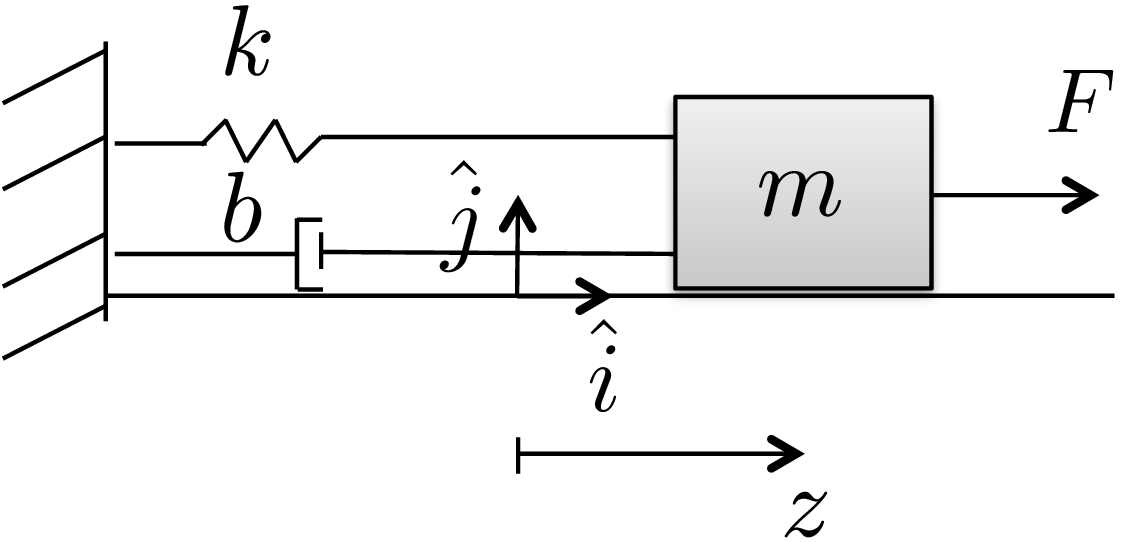
\includegraphics[width=0.5\textwidth]{6_design_studies/figures/hw_mass_kinetic_energy} 
   \caption{Computing the kinetic energy for the mass-spring-damper.}
   \label{fig:hw_mass_kinetic_energy}
\end{figure}
Define the inertial coordinate frame as in Figure~\ref{fig:hw_mass_kinetic_energy}, with $\hat{k}$ out of the page.  The horizontal position of the mass $m$ is given by 
\[
\mathbf{p} = \begin{pmatrix} z(t) \\ 0 \\ 0 \end{pmatrix}.
\]
Differentiating to obtain the velocity of $m$ 
\begin{align*}
\mathbf{v} = \begin{pmatrix}  \dot{z} \\ 0 \\ 0 \end{pmatrix}.
\end{align*}
Since there is no rotational motion of the mass, the 
kinetic energy of the system is given by
\begin{align}
K &= \frac{1}{2}m\mathbf{v}^\top\mathbf{v} \notag\\
  &= \frac{1}{2}m\begin{pmatrix} \dot{z} & 0 & 0 \end{pmatrix} \begin{pmatrix} \dot{z} \\ 0 \\ 0 \end{pmatrix} \notag\\
  &= \frac{1}{2}m\dot{z}^2.
  \label{eq:mass_kinetic_energy}
\end{align}





